\section{Published results}

  \begin{figure*}
    \centering
    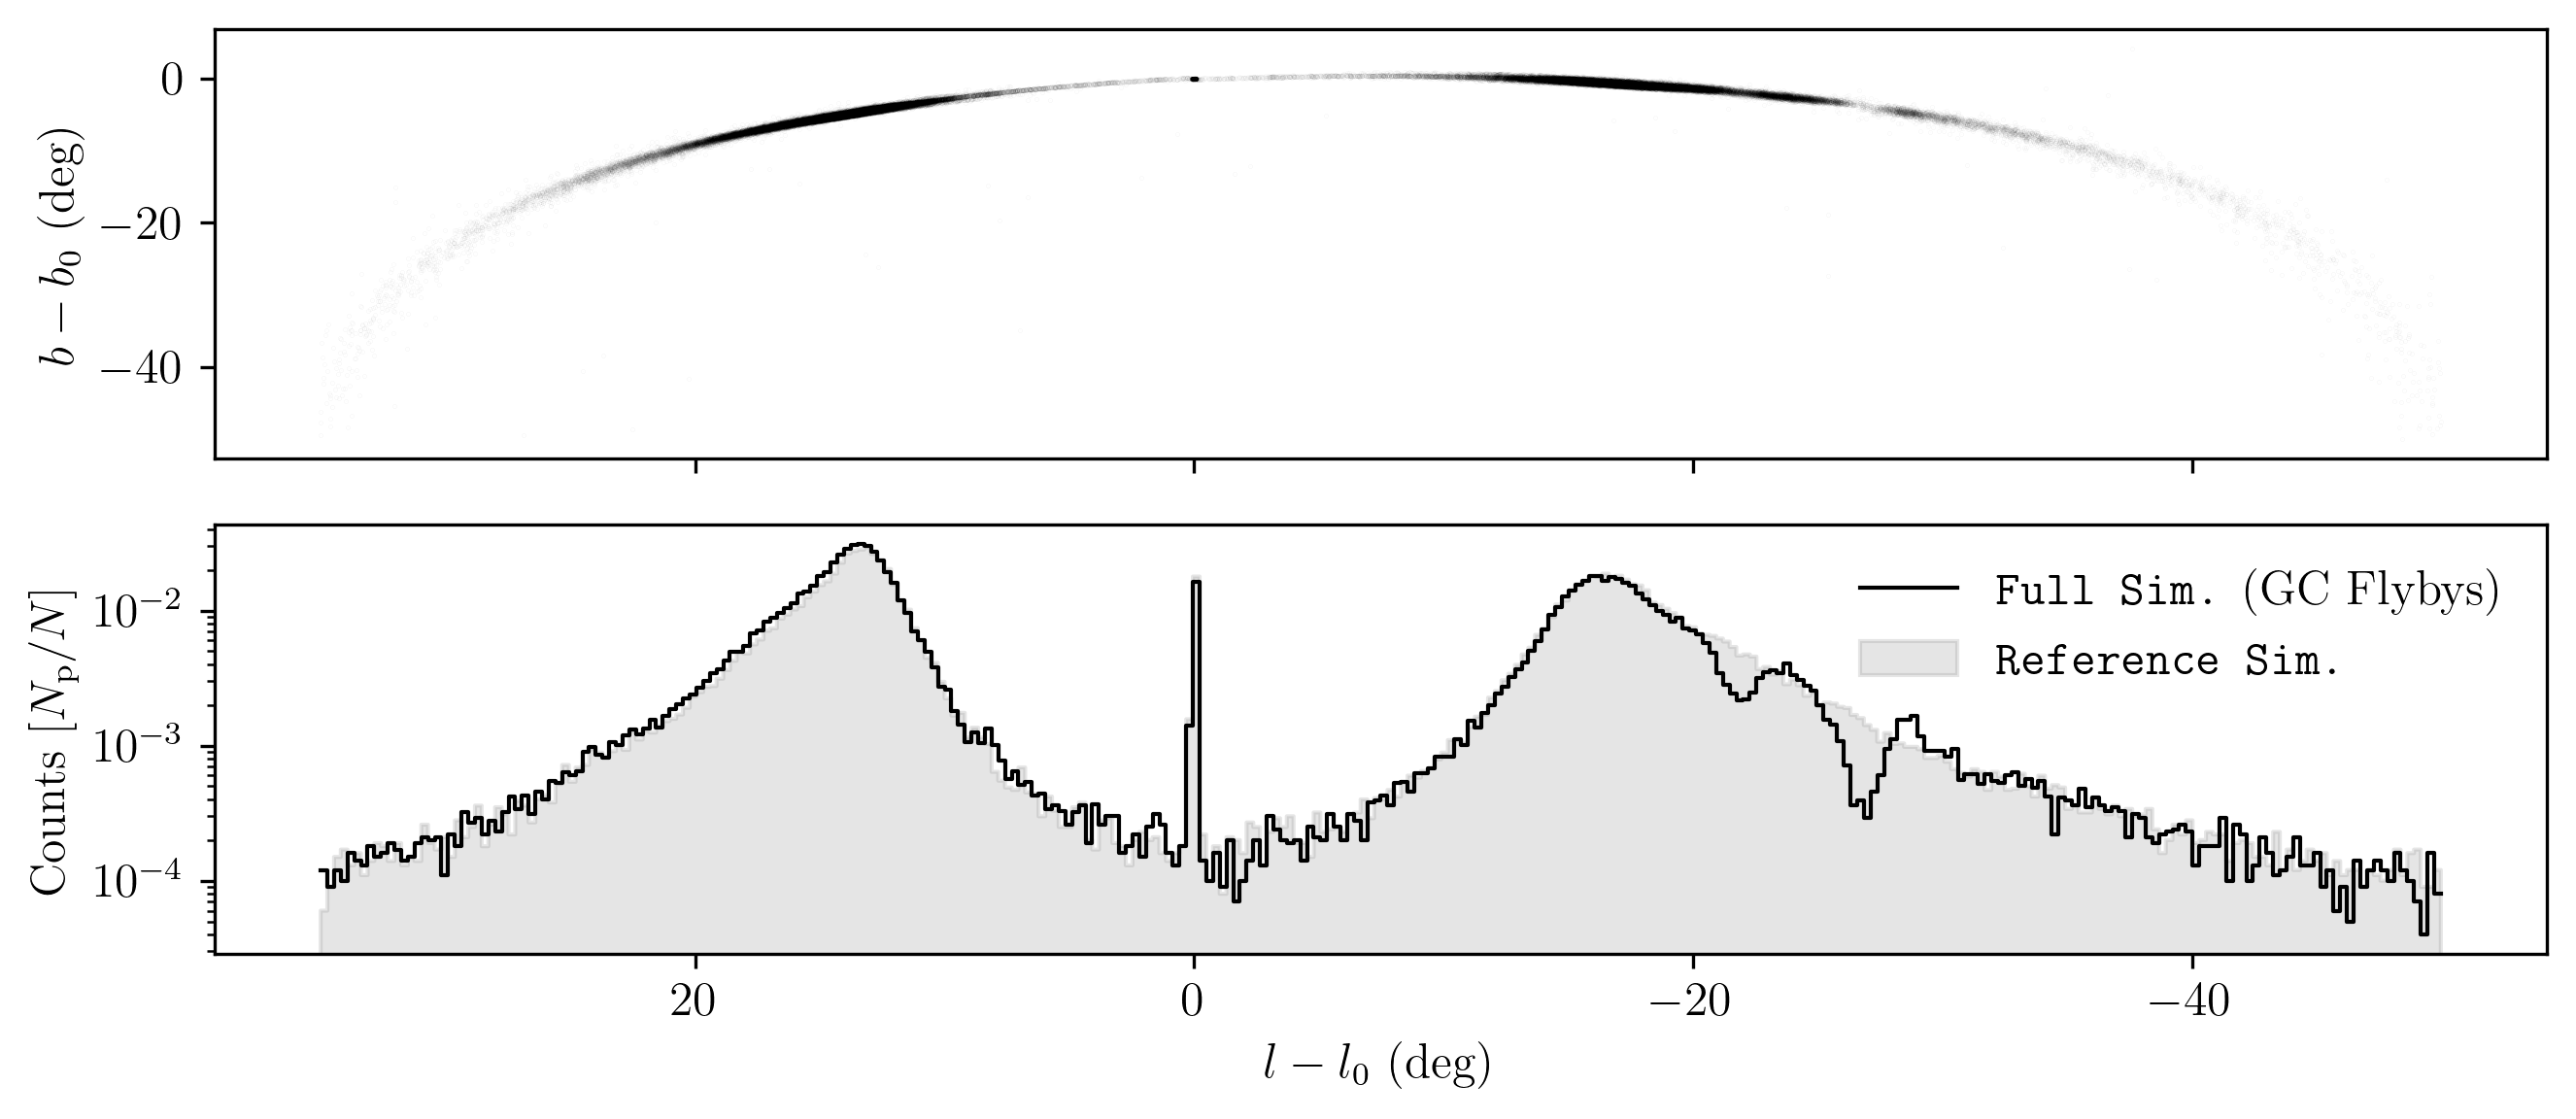
\includegraphics[width=\linewidth]{images/stream_on_sky_Pal5_monte-carlo-009_pouliasis2017pii-GCNBody_pouliasis2017pii.png}
    \caption{Simulated Palomar~5 stream created by modeling the host cluster as a Plummer sphere disrupting within an axis-symmetric Galactic potential plus the gravitational effect of 164 other Galactic globular clusters. The top panel shows the distribution of star particles that escaped the cluster due to tidal forces. The bottom panel shows the 1D density profile marginalized over longitude. The gray fill shows a reference simulation that uses the same conditions to produce the stream but does not include the other globular clusters. The large central peak in density is composed of particles still bound to Palomar~5. $\ell_0,b_0$ are located Palomar~5's cluster's center of mass. Two large gaps are present due to the passage of two globular clusters. $N_p$ indicates the number of particles in a bin, while $N$ is the total number of particles, which is 100,000.}
    \label{fig:stream_on_sky}
    \end{figure*}

\section{Methods}
    The most accurate model of the Palomar~5 stream would involve full modeling of the internal dynamics of the cluster, which would mean computing $N$-body interactions with a $\mathcal{O}(N^2)$ computation time, stellar evolution, supernovae, an initial mass distribution, treatment of binary star systems, etc. \citep[for such an example, see][]{2021NatAs...5..957G, 2016MNRAS.458.1450W}. Instead, we opt for solving the restricted-three-body problem, also known as the particle-test method, as we did for \citet{2023A&A...673A..44F}, which we describe here for completeness. As demonstrated by \citet{2012A&A...546L...7M}, although the restricted three-body problem neglects the internal evolution of the cluster, it still reproduces very similar stream properties since the model captures key extracluster physics, such as disk shocking and epicyclic stripping.\\

    Below, we first present the approach used to include the Galactic globular cluster system in our modeling (Sect.~\ref{numerical_meth}), highlighting the similarities and differences with respect to what we did in \citet{2023A&A...673A..44F}; we then summarize the method used to model the mass loss from the cluster (Sect.~\ref{sec:mass_loss}) and finally discuss the quality of the numerical integration (Sect.~\ref{num_quality}). 

    \subsection{Numerical methodology}\label{numerical_meth}
        We begin by extracting positions in the sky, proper motions, line-of-sight velocities, and distances, as well as masses and half-mass radii, of 165 globular clusters from the Galactic globular cluster catalog by \cite{2021MNRAS.505.5957B}.\footnote{The Baumgardt catalog has been assembled across a series of works, see: \cite{2020PASA...37...46B,2019MNRAS.482.5138B,2018MNRAS.478.1520B}. The catalog can be found on the World Wide Web at \href{https://people.smp.uq.edu.au/HolgerBaumgardt/globular/}{https://people.smp.uq.edu.au/HolgerBaumgardt/globular/}.} We then convert the initial conditions from sky coordinates into a Galactocentric reference frame, by adopting a velocity for the local standard of rest of $v_{\text{LSR}} = 240$~km~s$^{-1}$ and a peculiar velocity of the Sun equal to $(U_\odot, V_\odot, W_\odot)=(11.1, 12.24, 7.25)$~km~s$^{-1}$, as reported by \citet{2012MNRAS.427..274S}.  We set the Sun's position to $(x_\odot,y_\odot,z_\odot) = (-8.34,0,0.027)$~kpc. We took the vertical position above the disk from \citet{2001ApJ...553..184C} and the distance of the Sun to the Galactic center from \citet{2014ApJ...783..130R}. These transformations were performed using \texttt{astropy} \citep{2013A&A...558A..33A}.

        For the Galactic potential, we employed the second model from \citet{2017A&A...598A..66P}, a superposition of a thin disk, thick disk, and dark matter halo, with masses and scale lengths provided in Table~1 of \citet{2023A&A...673A..44F}. This model is time-independent throughout our simulations. This model satisfies a series of observational constraints such as local solar, stellar density, the Galactic rotation curve, similarly to other Galactic models such as \texttt{MWpotential2014} from \citet{2015ApJS..216...29B} and \texttt{McMillian2017} from \citet{2017MNRAS.465...76M}. However, we use only one Galactic potential to balance data volume and computation time, which should suffice. \citet{2021MNRAS.505.5978V} found that only a few outer globular clusters are strongly affected by different potential models. Generally, kinematic uncertainties are the dominant factor in differences between orbital solutions per cluster. Similarly, \citet{2024MNRAS.528.5189G} generated a globular cluster mass-loss catalog using seven different potential models and found that their debris distributions were rather model-independent, similar to those of \citet{2023A&A...673A..44F}. While the clusters' exact positions in time may depend on the model, we assert that interaction rates and stream formation are largely independent of the choice of the Galactic potential model.
    
        Lastly, we select an integration time of 5~Gyr as a compromise between maximizing interaction statistics and modeling the Galaxy as a time-independent, constant mass distribution. \citet{2023A&A...673A.152I} analyzed the orbits of the Galactic cluster population using the same initial conditions as in this work within five live Milky Way-like potentials from IllustrisTNG \citep{2018MNRAS.473.4077P}. They found that in all sampled potentials, orbital changes remain minimal over 5~Gyr, becoming significant only at earlier look-back times when the host galaxy had significantly less mass or was undergoing a merger event.


        \subsubsection{ \texttt{Full} simulations}
            There is a primary methodological departure from \citet{2023A&A...673A..44F}.  In that work, globular clusters evolved under the gravitational effect of the Galaxy alone. In contrast, now we also consider the effect of all other Galactic globular clusters by taking into account the direct $N$-body interactions between them. First, all clusters are represented by Plummer spheres, each with its own mass and half-mass radius as reported in the Baumgardt catalog \citep{2021MNRAS.505.5957B}. For the remainder of this paper, the \texttt{full} simulations consider the gravitational forces from the globular cluster interactions. \\
            For these simulations, we proceeded in two steps:
            \begin{enumerate}
                \item First, starting from the Galactocentric positions and velocities of all 165 Galactic globular clusters, we integrate their orbits back in time for 5~Gyr under the influence of the Galaxy itself and their mutual influence. In the backward integration, the system of equations of motion for the globular clusters is thus: 
                \begin{equation}
                    \ddot{\vec{r}}_i = -\nabla \Phi + \left.\sum_{j\neq i}^{N_{GC}} \frac{Gm_j}{\left(|\vec{r}_j - \vec{r}_i|^2 + b_j^2\right)^{3/2}}\right. \left(\vec{r}_j - \vec{r}_i\right),
                \end{equation}\label{eq:GCNBody} 
                \noindent where $\vec{r}$ indicates the Galactocentric position vector, the index $i$ indicates the globular cluster of interest; the index $j$ indicates the other globular clusters that are summed over. $N_{GC}$ is the total number of globular clusters, which in this study is 165, $m_j$ is the mass of the j-th cluster in the sample, $b_j$ is its Plummer scale radius, and $\vec{r_j}$ is its Galactocentric position. $\Phi$ represents the same Galactic smooth potential that we discussed previously \citep[][Model~II, in the present case]{2017A&A...598A..66P}. Note that the masses and sizes of the globular clusters are kept constant in these simulations and are not allowed to vary with time, which means that we do not consider their internal evolution. In sec.~\ref{sec:discussion}, we discuss the implications of the modeling limitations.
                \item Once we found the positions and velocities of the entire globular cluster, we sampled Palomar~5 with 100,000 particles from a Plummer distribution, taking the mass and half-mass radius from the Baumgardt catalog: $1.3\times10^{4}~\textrm{M}_\odot$ and $27.6~\textrm{pc}$. We then integrated the evolution of these particles forward in time to the present day, taking into account that each particle feels the gravitational potential of the Galaxy, its host cluster, and that of all the other clusters in the Galaxy. Note that we do not account for self-gravity among particles. The particles experience the gravitational field yet do not contribute to it, a common assumption in galactic dynamics, as the mass of an individual star is negligible compared to the mass of the larger dynamical system. The equation of motion of a generic particle among the 100,000 that populate Palomar~5 is thus: 
                \begin{equation}
                    \ddot{\vec{r}}_p = -\nabla \Phi + \left.\sum_{j}^{N_{GC}} \frac{Gm_j}{\left(|\vec{r}_j(t) - \vec{r}_p|^2 + b_j^2\right)^{3/2}}\right. \left(\vec{r}_j(t)- \vec{r}_p\right),
                \end{equation} \label{eq:equation_of_motion_particle} where the index $p$ represents one of the 100,000 particles of interest, $\vec{r_p}$ being its position, and $j$ indexes over the globular clusters as in Eq.~\ref{eq:GCNBody}. We note that in Eq.~\ref{eq:equation_of_motion_particle}, the positions of the globular clusters are time-dependent since they are being loaded during this step and not computed, unlike Eq.~\ref{eq:GCNBody}. 
            \end{enumerate}

            The procedure described so far has been repeated 50 times, generating a new set of initial conditions each time, given the uncertainties on proper motions, line-of-sight velocities, distances to the Sun, and masses of all clusters, as reported in the Baumgardt catalog. We handle these uncertainties through a Monte-Carlo approach by sampling them with a Gaussian distribution and considering the covariance term between the proper motions. We use the most probable values for the initial conditions in the first simulation. We sample the uncertainties for all globular clusters. Additionally, for each resampling of Palomar~5's mass, we also resample the distribution of the 100,000 star particles. 

            During the integration, we save intermediate snapshots to facilitate the analysis of stellar streams and the effects of cluster impacts. Specifically, for each realization of the Palomar~5 stream, we saved $5000$ in snapshots, equivalent to a temporal resolution of 1 million years. We provide the parameters that specify our data volume in Table~\ref{tab:data_volume}. Using single precision floating point numbers, the size of our simulations is approximately:
            \begin{equation} \label{eq:data_volume_estimate}
                N_p \times N_{\textrm{ts}}\times N_{\textrm{phase}}\times N_{\textrm{sampling}} \times 4~\textrm{bytes}\approx 600~\textrm{Gb}.
            \end{equation}

            \begin{center}
                \begin{table}[h]
                    \centering
                    \caption{Parameters determining the data volume.}
                    \label{tab:data_volume}
                    \begin{tabular}{|c|c|c|c|}
                        \hline
                        $N_p$ & $N_{\textrm{ts}}$ & $N_{\textrm{phase}}$ & $N_{\textrm{sampling}}$ \\
                        \hline
                        $100000$ & $5000$ & $6$ & $50$ \\
                        \hline
                    \end{tabular}
                    \tablefoot{$N_p$  is the number of particles, $N_{\textrm{ts}}$ is the number of time-steps saved, $N_{\textrm{phase}}$ is the number of phase space coordinates, and $N_{\textrm{sampling}}$ is the number of Monte-Carlo samplings of the initial conditions.}
                \end{table}
            \end{center}

        \subsubsection{ \texttt{Reference} simulations}
        To quantify the impact of globular cluster passages on the density of the Palomar~5 stream, we performed a second set of simulations, which we refer to as the \texttt{reference} simulations in this paper.  These \texttt{reference} simulations use the same 50 sets of initial conditions as the \texttt{full} simulations, the same Galactic potential, but exclude mutual interactions between globular clusters. The approach adopted for this second set of simulations is thus equivalent to that adopted already in \citet{2023A&A...673A..44F}. In Eq.~\ref{eq:GCNBody}, only the gradient of the Galactic potential is considered. In Eq.~\ref{eq:equation_of_motion_particle}, of the second term on the right side of the equation, only the influence of Palomar~5's Plummer sphere on Palomar~5's particles is considered. In other words, the sum iterates over only one globular cluster, the host. We omit all interactions with the other clusters.
    \subsection{Mass loss}\label{sec:mass_loss}

        Each of the 100,000 particles that initially populate the cluster undergoes experiences the forces from Pal~5 and the Galactic potential. The mass and radius of Pal~5 are held constant over time. At each time step, a certain number of particles will therefore acquire sufficient energy to no longer be gravitationally bound to the cluster itself and thus go on to populate the streams, whose mass and spatial extent grow over time. It is important to note that in the approach used:

        \begin{enumerate}
            \item The masses and sizes of the clusters (and therefore the parameters of the Plummer potentials) do not change over time, which is an oversimplification, because in a self-consistent approach, these parameters would vary. 
            \item We use the same initial conditions for Pal~5 progenitor as it has today, and this is also a simplification, since Pal~5 - 5 Gyr years ago - must have contained at least part of the mass estimated today in its tails\footnote{We used the same approach (i.e., time-independent masses and sizes) to model the whole set of globular clusters.}. 
        \end{enumerate}

        The assumption in point 2 is a direct consequence of the approach described in point 1. Starting from a cluster with a mass and size similar to the current ones can lead to streams with lower velocity dispersions than those we would obtain if we had used a self-consistent approach. In a future article, we will report on the study of gap survival times depending on the masses and sizes of progenitor clusters (Ferrone et al, in prep). We note, however, that simplifications of this kind are not uncommon in literature. \citet{2017NatAs...1..633P} discussed the formation of gaps in the Pal~5 tails and assumed a time-independent mass of $50,000 ~\textrm{M}_\odot$ for Pal~5, over the last 4~Gyr; \citet{2017MNRAS.470...60E} adopted a N-body approach to simulate Pal~5 stream, but used Pal~5 current conditions as their progenitor's initial conditions; \citet{2019MNRAS.484.2009B} simulated the Pal~5 stream as emerging from a stellar system with a velocity dispersion of 0.5~km/s (similar to that of particles escaping from our cluster, as we have verified). 

        The characteristics of the streams modeled in this paper may be considered more representative of those of clusters that are now completely dispersed, i.e., it is conceivable that completely dispersed globular clusters that left behind a population of `orphan' streams passed through characteristics similar to those of Pal 5~today (small masses and extended radii). In this sense, the initial conditions chosen (in terms of internal parameters) may be more representative of those of streams for which the progenitor is now dissolved \citep[see, for example, the population of streams without progenitors described by][]{2024ApJ...967...89I} than those currently typical of Galactic globular clusters than those currently typical of Galactic globular clusters. \footnote{In this regard, we recall that \citet{2014ApJ...795...95B} modeled the GD-1 stream as the result of the dissolution of a cluster with a mass of $2 \times 10^4 M_\odot$, and a tidal radius of $0.07$~kpc.}


    \subsection{Numerical stability}\label{num_quality}

        We used a leapfrog integrator because of its ability to preserve phase-space volume and conserve the Hamiltonian with each integration step. For instance, this method is preferable to a Runge-Kutta scheme, which can introduce non-physical and significant numerical errors in systems that require long-term stability and energy conservation. One drawback of the leapfrog integrator is that it requires a uniform time step throughout the entire computation, resulting in unnecessary computations for a particle after it has escaped from the host cluster. However, energy conservation and phase-space volume preservation are paramount when modeling stellar streams. The time step was therefore set to be small enough to conserve energy for the most interior particles within the cluster---ensuring that a higher mass loss did not arise from numerical error. We found that a time-step of 10,000 years was adequate to maintain energy conservation, with a median variation of $10^{-12} \frac{\Delta E}{E_0}$, where $E_0$ is a particle's initial energy, and $\Delta E$ is the difference between its final and initial energy. 
    
        We also checked the reverse integrability of the globular cluster system for the \texttt{reference} simulations. By reverse integrability, we mean the integrator's capability to track the cluster backward in time and then re-integrate it forward along the same trajectory. Integrating point masses in a static axis-symmetric potential conserves $L_z$ and $E$, which create regular periodic and non-chaotic orbits. Therefore, any drift would arise from purely numerical error. We selected a timestamp for which the drift in the final position after forward integration, compared to the initial position from the backward integration, was consistently at least two orders of magnitude smaller than the Plummer scale radius used for Palomar~5. This high precision ensures that no fictitious numerical forces influence the system, preventing any artificial mass loss or retention of star particles.



\section{Results}

    \subsection{Overview}
        \begin{figure*}
            \centering
            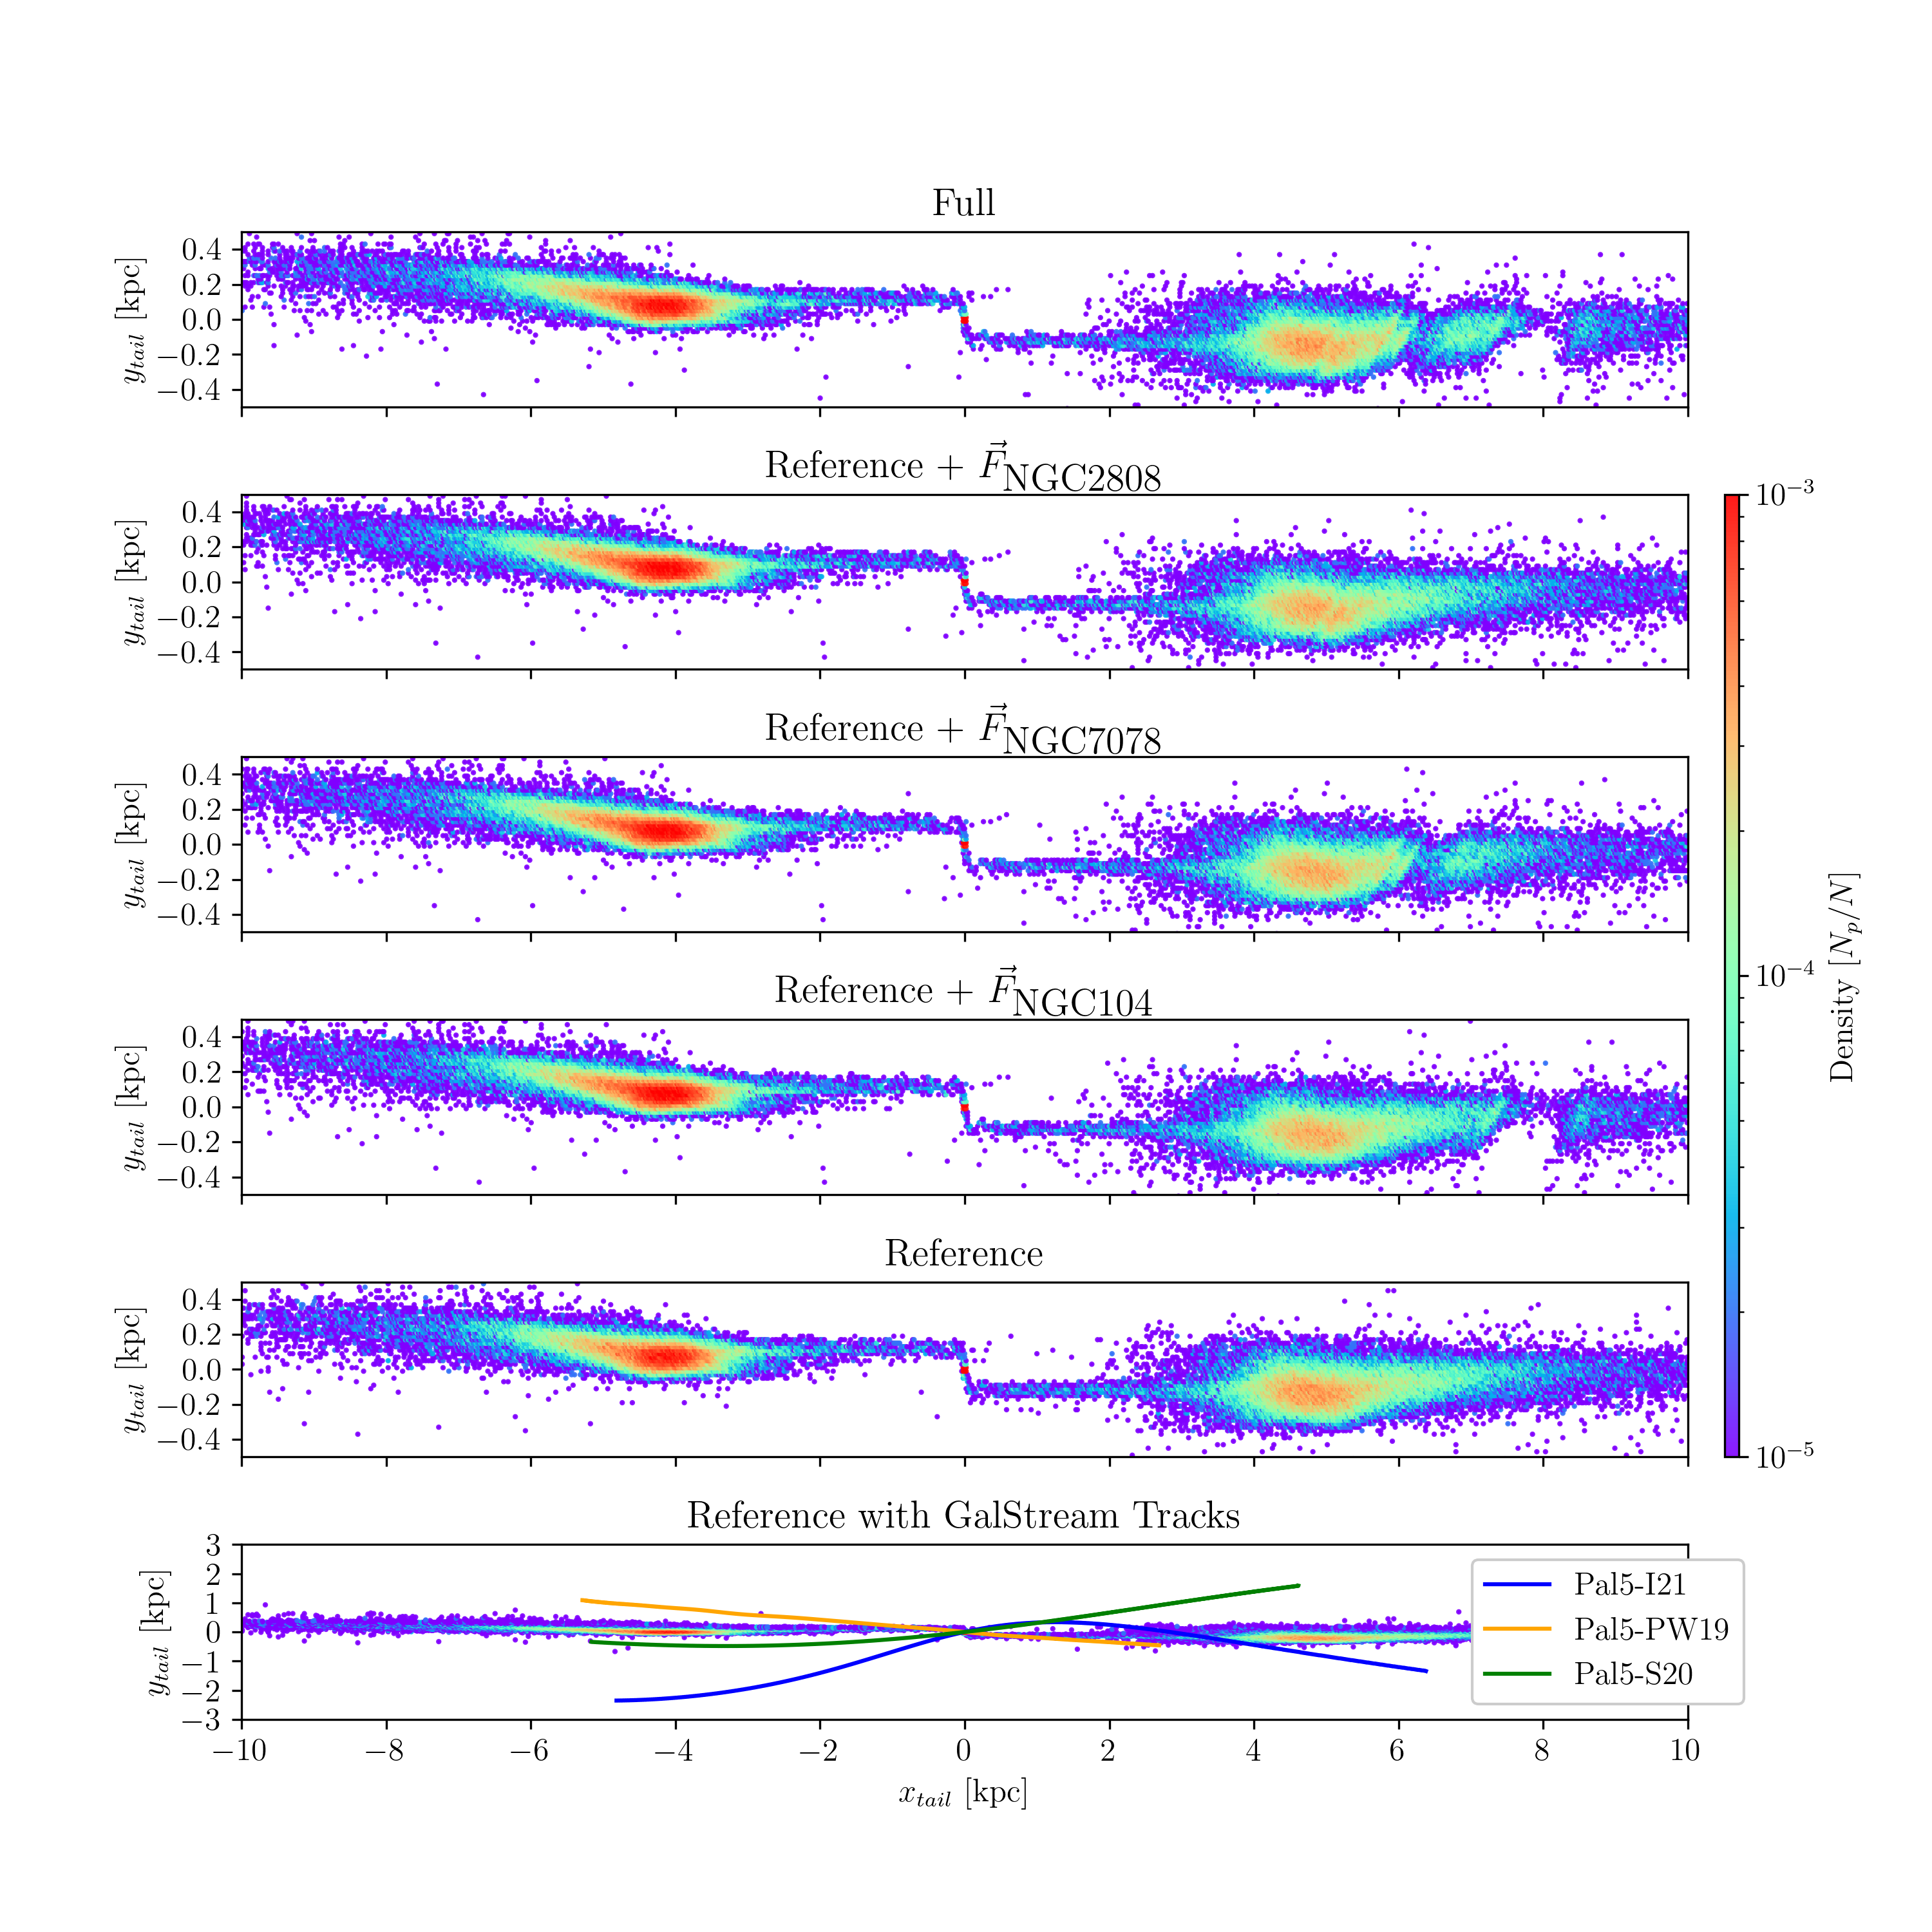
\includegraphics[width=\linewidth]{images/decomposition-monte-carlo-009-with-3-gaps-domidpoint-shift.png}
            \caption{Density maps of Palomar~5's stream in the tail coordinate system, where $x\prime$ is the integrated arc length along the cluster's orbit and $y\prime$ is the distance within the orbital plane. The color scale represents normalized particle counts (total: 100,000). The top panel shows the \texttt{full} simulation with three gaps on the stream's right-hand side. The next three panels depict simulations with identical initial conditions but exclude the gravitational influence of all clusters except those forming a given gap. The \texttt{Reference} simulation omits the influence from other globular clusters. The bottom panel compares Palomar~5's observed stream length to the \texttt{Reference} simulation, using the same Monte-Carlo realization as Fig.~\ref{fig:stream_on_sky} and \texttt{Sampling~009} (as seen in the \href{https://doi.org/10.5281/zenodo.15528089}{online appendix}).}
            \label{fig:decomposition}
        \end{figure*} 
    
        \begin{figure*}
            \centering
            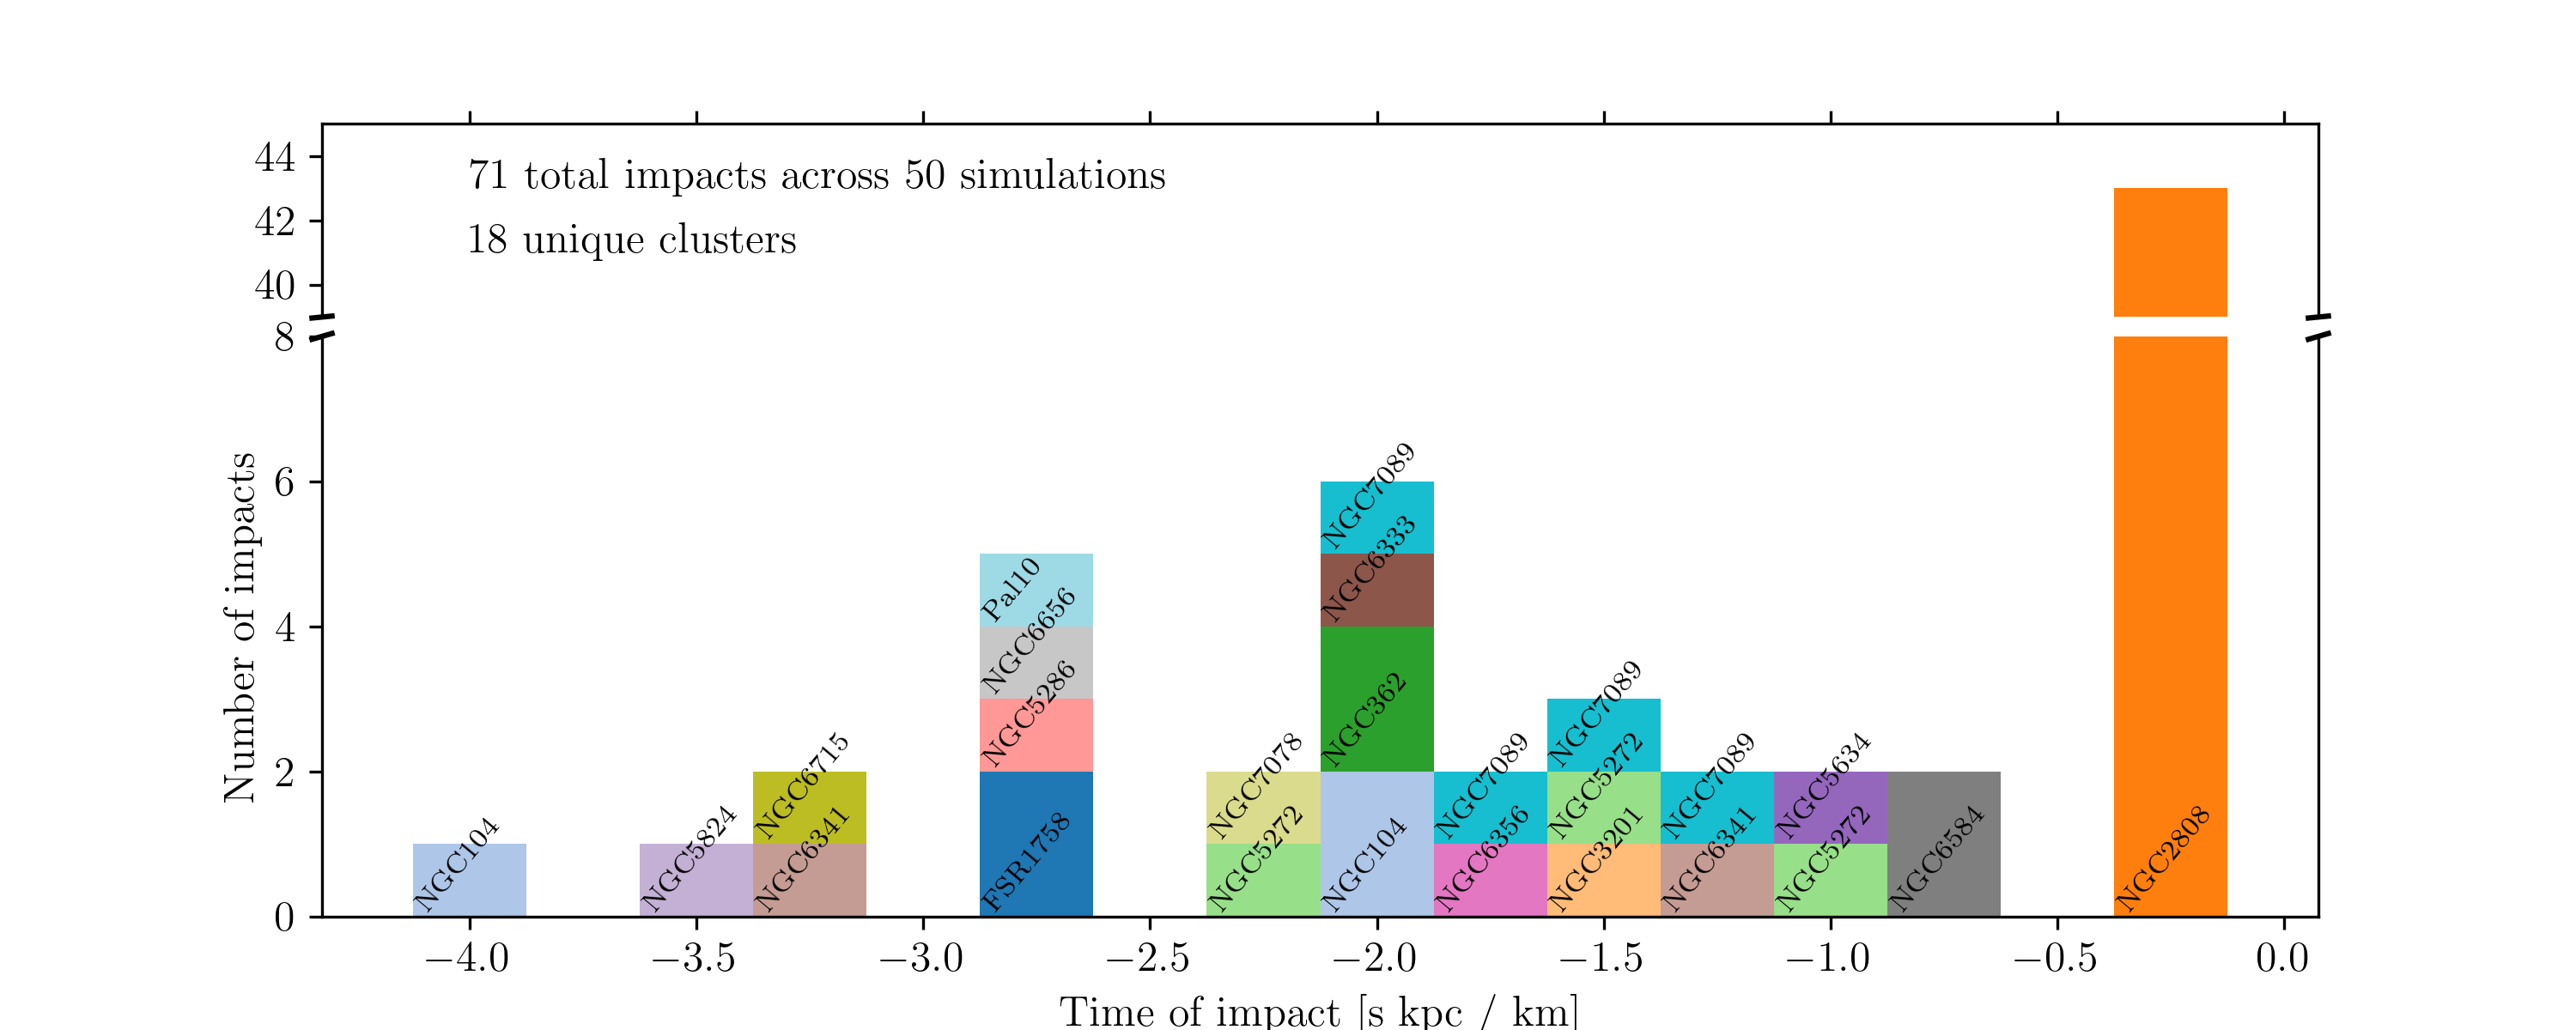
\includegraphics[width=\linewidth]{images/histogram_impact_time.png}
            \caption{Simulation time when the impacts occurred for all gap-causing flybys summed over all 50 simulations. Each perturbing cluster is labeled and color-consistent. We report the time axis in simulation units, with 1~s~kpc~km~$^{-1}$ corresponding to roughly 1~Gyr. We note that the plot breaks the y-axis to accommodate the large number of encounters from NGC~2808 without overshadowing the other interactions.}
            \label{fig:histogram_impact_time}
        \end{figure*}

        The presence of the other globular clusters affects the properties of the Palomar~5 stream. Fig.~\ref{fig:stream_on_sky} presents an obvious example of this effect, which we selected for its prominent gaps. Two of these gaps are visible in Galactic coordinates and become even more apparent when marginalizing over latitude to reconstruct the 1D density profile of the stream as a function of longitude.     

        Regarding the shape of the density distribution, the central peak corresponds to the still-intact globular cluster whose stars have not yet escaped. The stream's density peaks are of the same order as the cluster itself, which is inconsistent with reality; the cluster's peak density should be higher than that of the stream. Of course, this discrepancy is a result of our modeling choices. Since we use the present-day mass and radius for Palomar~5 for the whole simulation duration, the system is less dense than it should have been. In turn, our simulations have a strong initial mass loss, which adds to the amplitudes of the profile density peaks of Fig.~\ref{fig:stream_on_sky}. This inaccuracy is acceptable for the scope of this work. First, Palomar~5's tails indeed have more mass than the cluster itself. \citet{2017ApJ...842..120I} reports that there could be three times as much mass in Palomar~5's tails as the cluster itself. Secondly, the exact form of the density distribution is less important than having a population of particles present that can probe a cluster flyby event.
    
        To compare the \texttt{reference} and \texttt{full} simulations more quantitatively, we work in the tail coordinate system, in which the stream's central axis aligns with the cluster's orbit. We based this coordinate system on the work of \citet{2004AJ....127.2753D} and present it in Fig.~\ref{fig:TailCoordinates}. Briefly, in this system, the $x_{\textrm{tail}}$ coordinate represents the position of a particle along the orbit relative to the globular cluster. Positive values of $x_{\textrm{tail}}$ are ahead of the cluster, while negative $x_{\textrm{tail}}$ is behind the cluster. The $y_{\textrm{tail}}$ coordinate measures the particle's distance within the orbital plane, where positive values indicate that the particle is farther from the Galactic center and negative values indicate that it is closer. Fig.~\ref{fig:decomposition} shows a comparison between one of the 50 realizations of the Palomar~5 stream, taking into account the gravitational interactions with all other globular clusters in the Galaxy (top panel) and omitting them (bottom panel). This comparison clearly shows the presence of two wide ($\sim$100~pc and $\sim$1~kpc) gaps in the leading tail and of a more subtle underdensity at $x_{\textrm{tail}}\sim 5$~kpc (we refer the reader to Appendix~\ref{sec:gap_detection} for a detailed description of the underdensities and gaps detection method). 
    
        To determine which globular clusters were responsible for creating these gaps and when close passages occurred, we estimated the gravitational acceleration along the orbit of Palomar~5. We represented it in the ($t$, $\tau$) space. $t$ is the simulation time, and $\tau$ indicates how long it will take for Palomar~5 to reach a given point in its orbit or how long ago it passed. The use of $\tau$ is advantageous because the growth of the stream is approximately linear in $\tau$. 
    
        On the other hand, streams in physical space are modulated by their orbital eccentricity with periodic expansion and contraction depending on the orbital phase \citep[see the top panel of Fig.~5.][for an example]{2016MNRAS.457.3817S}. Adopting this time-space and reporting the gravitational acceleration along the Palomar~5 orbit in this space, identifying the globular clusters that produced the perturbation and the time at which it occurred becomes straightforward. We refer the reader to Appendix~\ref{sec:Perturber_Identification} for a detailed description of the procedure. In this way, we can identify that the clusters responsible for creating gaps in the simulation of the Palomar~5 stream, as reported in Fig.~\ref{fig:decomposition}, are NGC~2808, NGC~7078, and NGC~104. Their close passages occurred 200~Myr, -1.9, and -2.1~Gyr ago, respectively. 
    
        To further investigate whether the three clusters above are responsible for producing the gaps observed in this simulation, we conducted additional experiments by including only the perturbation of each cluster at a time, while neglecting the gravitational perturbations of all the other clusters in the Galaxy.
    
        To verify that the three suspected clusters are responsible for producing the gaps, we conducted experiments by including one perturbed at a time and excluding all others. We present these results in the middle panels of Fig.~\ref{fig:decomposition} and clearly show that NGC~2808, NGC~7078, and NGC~104 are the clusters responsible for creating the underdense regions observed in the leading tails of Palomar~5. It is worth noting that the times at which the passages of these clusters occurred, according to our analysis, are in agreement with the observed width of the corresponding gaps: the encounter with NGC~2808 being very recent (only 200~Myr ago), its induced gap is still very thin, because it takes time for a perturbation to grow into an extended gap, as it is the case for those induced by the passages of  NGC~7078 and NGC~104, which occurred in earlier times. It is also interesting to emphasize that gaps as thin as those generated by the passage of NGC~2808, 200~Myr ago, can be detected by working in the tail coordinate system and by making a comparative analysis (\texttt{full} versus \texttt{reference} simulations): they are so thin that they cannot be directly identified in Galactic coordinates (see Fig.~\ref{fig:stream_on_sky}).\\

        The analysis presented in Fig.~\ref{fig:decomposition} has been repeated for the whole set of simulations, and \href{https://doi.org/10.5281/zenodo.15528089}{online appendix} reports all of them for completeness. For all the streams, morphologically speaking, the only changes appear to be the existence of gaps or their absence. We do not observe a thickening of the streams due to an increased velocity dispersion. 
    
        From this analysis, we can derive a statistical view of (1) the number of gaps generated on the Palomar~5 stream by the system of Galactic globular clusters, (2) the clusters that generated these gaps, and the time history of these perturbations. From this, we can then quantify (3) the properties of the perturbers (their masses, sizes, and orbital parameters) as well as (4) the impact geometry of the encounters, which allows us to understand which encounters are more favorable for generating gaps in the Palomar~5 stream. In the following, we will present the results of this analysis, addressing points (1) and (2).


    \subsection{The history and statistics of gap creations in the Palomar~5 stream}\label{sect:history}
        By applying the methodology described above to the whole set of simulations, we can reconstruct the history of close passages of Galactic globular clusters to Palomar~5's stream in the last 5~Gyr, which -- we remind the reader -- is the time interval investigated in our simulations.  Fig.~\ref{fig:histogram_impact_time} and Table~\ref{tab:gaps_per_perturber} present results of this analysis. NGC~2808 impacted Palomar~5's stream about 200 Myr ago in 44 out of 50 simulations, creating a small gap at a similar position to the one reported in Fig.~\ref{fig:decomposition} in each case. Since this interaction occurred less than one orbital period ago, despite the uncertainties, the orbital solutions remain similar and thus produce consistent results across all simulations. However, as we continue to turn back time further, the uncertainties in the initial conditions allow the various orbital solutions to diverge from one another. Thus, in one configuration, a cluster can impact the stream at a given time, and yet at the same moment, in a different set of initial conditions, it could be on the other side of the Galaxy. We will discuss the necessary conditions for creating a gap in Appendix~\ref{sec:gaps_vs_gcmass}. 
        \begin{table}[h]
            \centering
            \caption{Number of gaps created by each perturber across all 50 simulations.}
            \label{tab:gaps_per_perturber}
            \begin{tabular}{|ll|ll|ll|}
            \hline
            NGC2808 & 44 & NGC7089 & 5 & NGC5272 & 4 \\
            NGC6584 & 3 & NGC6341 & 2 & NGC6656 & 2 \\
            NGC104 & 2 & NGC3201 & 1 & NGC5634 & 1 \\
            NGC5286 & 1 & NGC362 & 1 & NGC5824 & 1 \\
            NGC6356 & 1 & NGC6333 & 1 & NGC6715 & 1 \\
            FSR1758 & 1 & NGC7078 & 1 & Pal10 & 1 \\
            \hline
            \end{tabular}
            \tablefoot{These data are color-coded and illustrated in Fig.~\ref{fig:histogram_impact_time}.}
        \end{table} 

        In total, we report the finding of 73 gaps across our 50 simulations, which averages to 1.5 gaps per simulation. Eighteen different perturbers provoke the gaps. Table~\ref{table:gap_distribution} presents the distribution of the number of gaps appearing per simulation. If we consider NGC~2808 an outlier and exclude it from the experiment, we observe an average of 0.6 gaps per simulation.  

        \begin{table}[h]
            \centering
            \caption{Occurrence of gaps in Palomar~5 streams, in our simulations.}\label{table:gap_distribution}
            \begin{tabular}{|l|c|c|c|c|c|}
                \hline
                Number of Gaps & 0 & 1 & 2 & 3 & 4 \\
                \hline
                Number of Sims. & 4 & 25 & 16 & 4 & 1 \\
                \hline
            \end{tabular}
            \vspace{0.5cm}
            \tablefoot{More specifically, the table reports the number of simulations (second row) for a given number of gaps (first row).}
        \end{table}

        We need a more sophisticated statistic to compare our results to other simulations, so we turn to the gap creation rate developed by \citet{2012ApJ...748...20C}. The gap creation rate is the number of gaps that appear per unit time and is normalized by the stream's length. For our simulations, this rate is given by: \begin{equation} \label{eq:gap_creation_rate} \mathcal{R}_{\textrm{Pal 5}} =  \frac{1}{T}\int_{0}^T l^{-1}(t) \sum_i \delta(t-t_i) dt,\end{equation}where $T$ is the total integration time, $l(t)$ is the length of the stream, and $\sum_i \delta(t-t_i)$ sums over the gap occurrences, with $i$ indexing over the number of gaps in a given simulation. Here, $\delta$ represents the Dirac delta function. This expression can be simplified to:\begin{equation}\mathcal{R}_{\textrm{Pal 5}} =  \frac{1}{T} \sum_i \frac{1}{l (t_i)}. \end{equation}
        
        This computation allowed us to analyze the distribution of gap creation rates across all simulations. Notice that since the gap creation rate adds in parallel, naturally, gaps that occur at earlier times when the stream was shorter are weighted higher than those that occur when the stream is longer. Fig.~\ref{fig:gapcreationrate} presents these results which are is roughly consistent with a simple estimate of the average gap creation rate: with 73 gaps over 5~Gyr of integration time for a stream about 20 kpc in length, the naive estimate is approximately 0.015~km~s$^{-1}$~kpc$^{-2} $ (which is roughly equivalent to $0.015~\rm{Gyr^{-1}kpc^{-1}}$). This naive estimate is about double the weighted mean gap creation rate of 0.009~km~s$^{-1}$~kpc$^{-2}$ and is higher because it does not account for the growth of the stream over time, unlike Eq.~\ref{eq:gap_creation_rate}.

        \begin{figure}
            \centering
            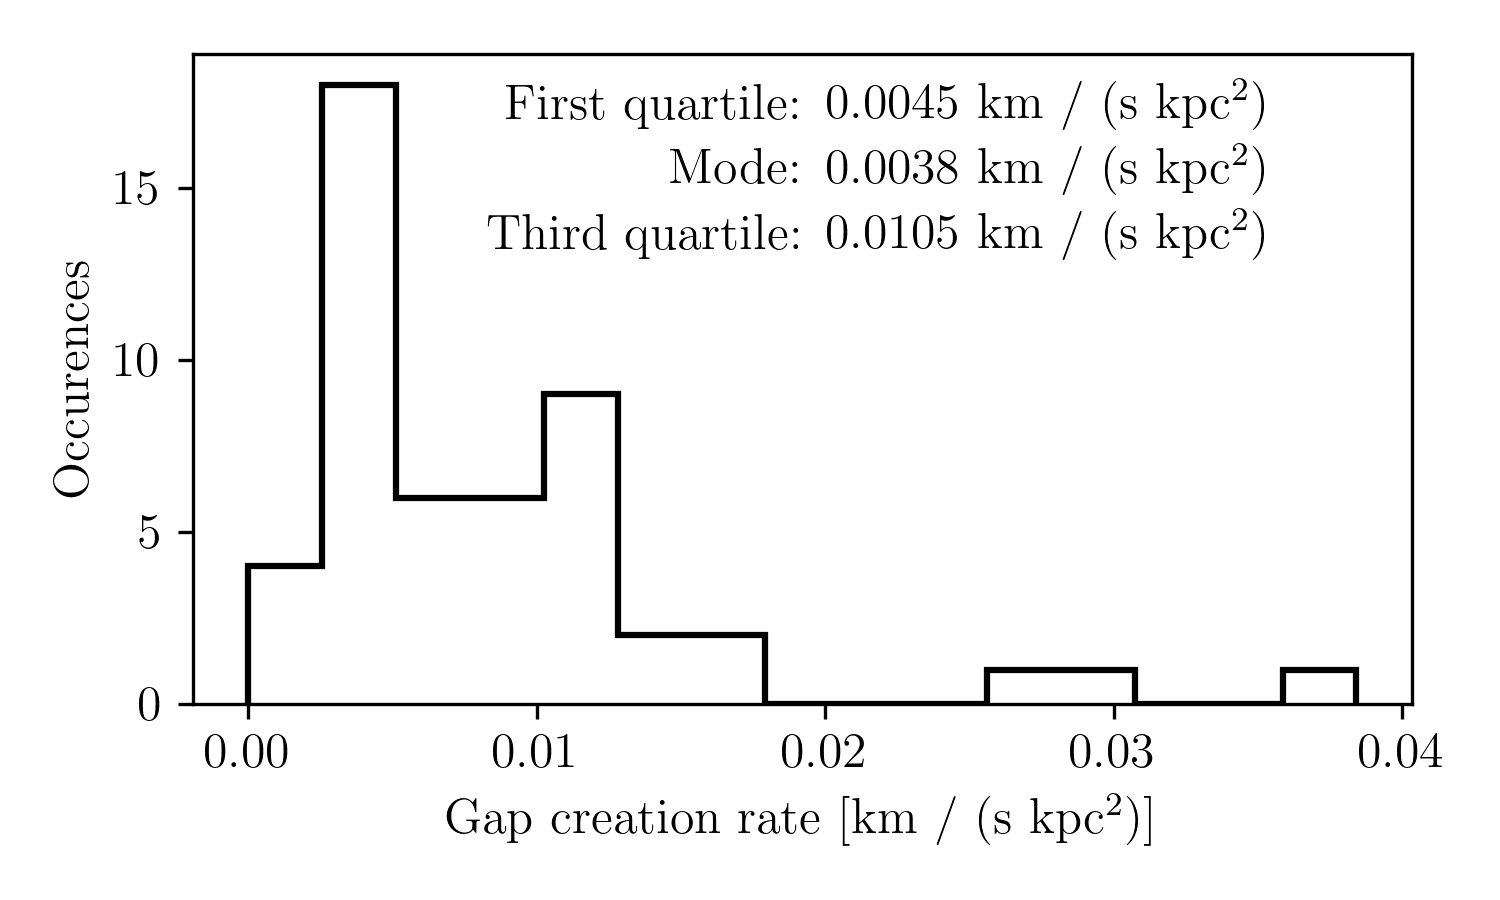
\includegraphics[width=\linewidth]{images/gap_creation_rate.png}
            \caption{Distribution of the number of gaps normalized over the total integration time and unit stream length as described by Eq.~\ref{eq:gap_creation_rate} for the whole set of 50 \texttt{full} simulations. }
            \label{fig:gapcreationrate}
        \end{figure}

        Lastly, we note that of the 73 observed gaps, only eight are in the trailing tail, and the rest are in the leading tail, which is a surprising result. A priori, since the star particles escape at similar rates from the L$_1$ and L$_2$ Lagrange points, each tail is of similar length and density. The main difference between the two tails is that the leading tail is closer to the Galactic center than the trailing tail by about 400~pc. Since the lengths are equal, and the offset between the tails is slight compared to the Galactocentric distance of about 10~kpc, we expected the gaps in each tail to be more or less the same. We can compute the probability of observing the unequal occurrences through the binomial distribution. First, since the 44 gaps linked to NGC~2808 are the result of the same flyby, they are not independent events. We remove them from this consideration, which leaves 21 gaps in the leading tail and 8 in the trailing. The probability of observing up to 8 successes in 29 trials, given a 50\% chance of success, is 1.2\%--unlikely, but possible. Additionally, other perturbers impact at consistent times, which may violate the assumption of independent events, as seen with NGC~2808.

    \subsection{Impact geometry and parameters of the perturbers}\label{sect:geometry}

        \begin{figure*}
            \centering
            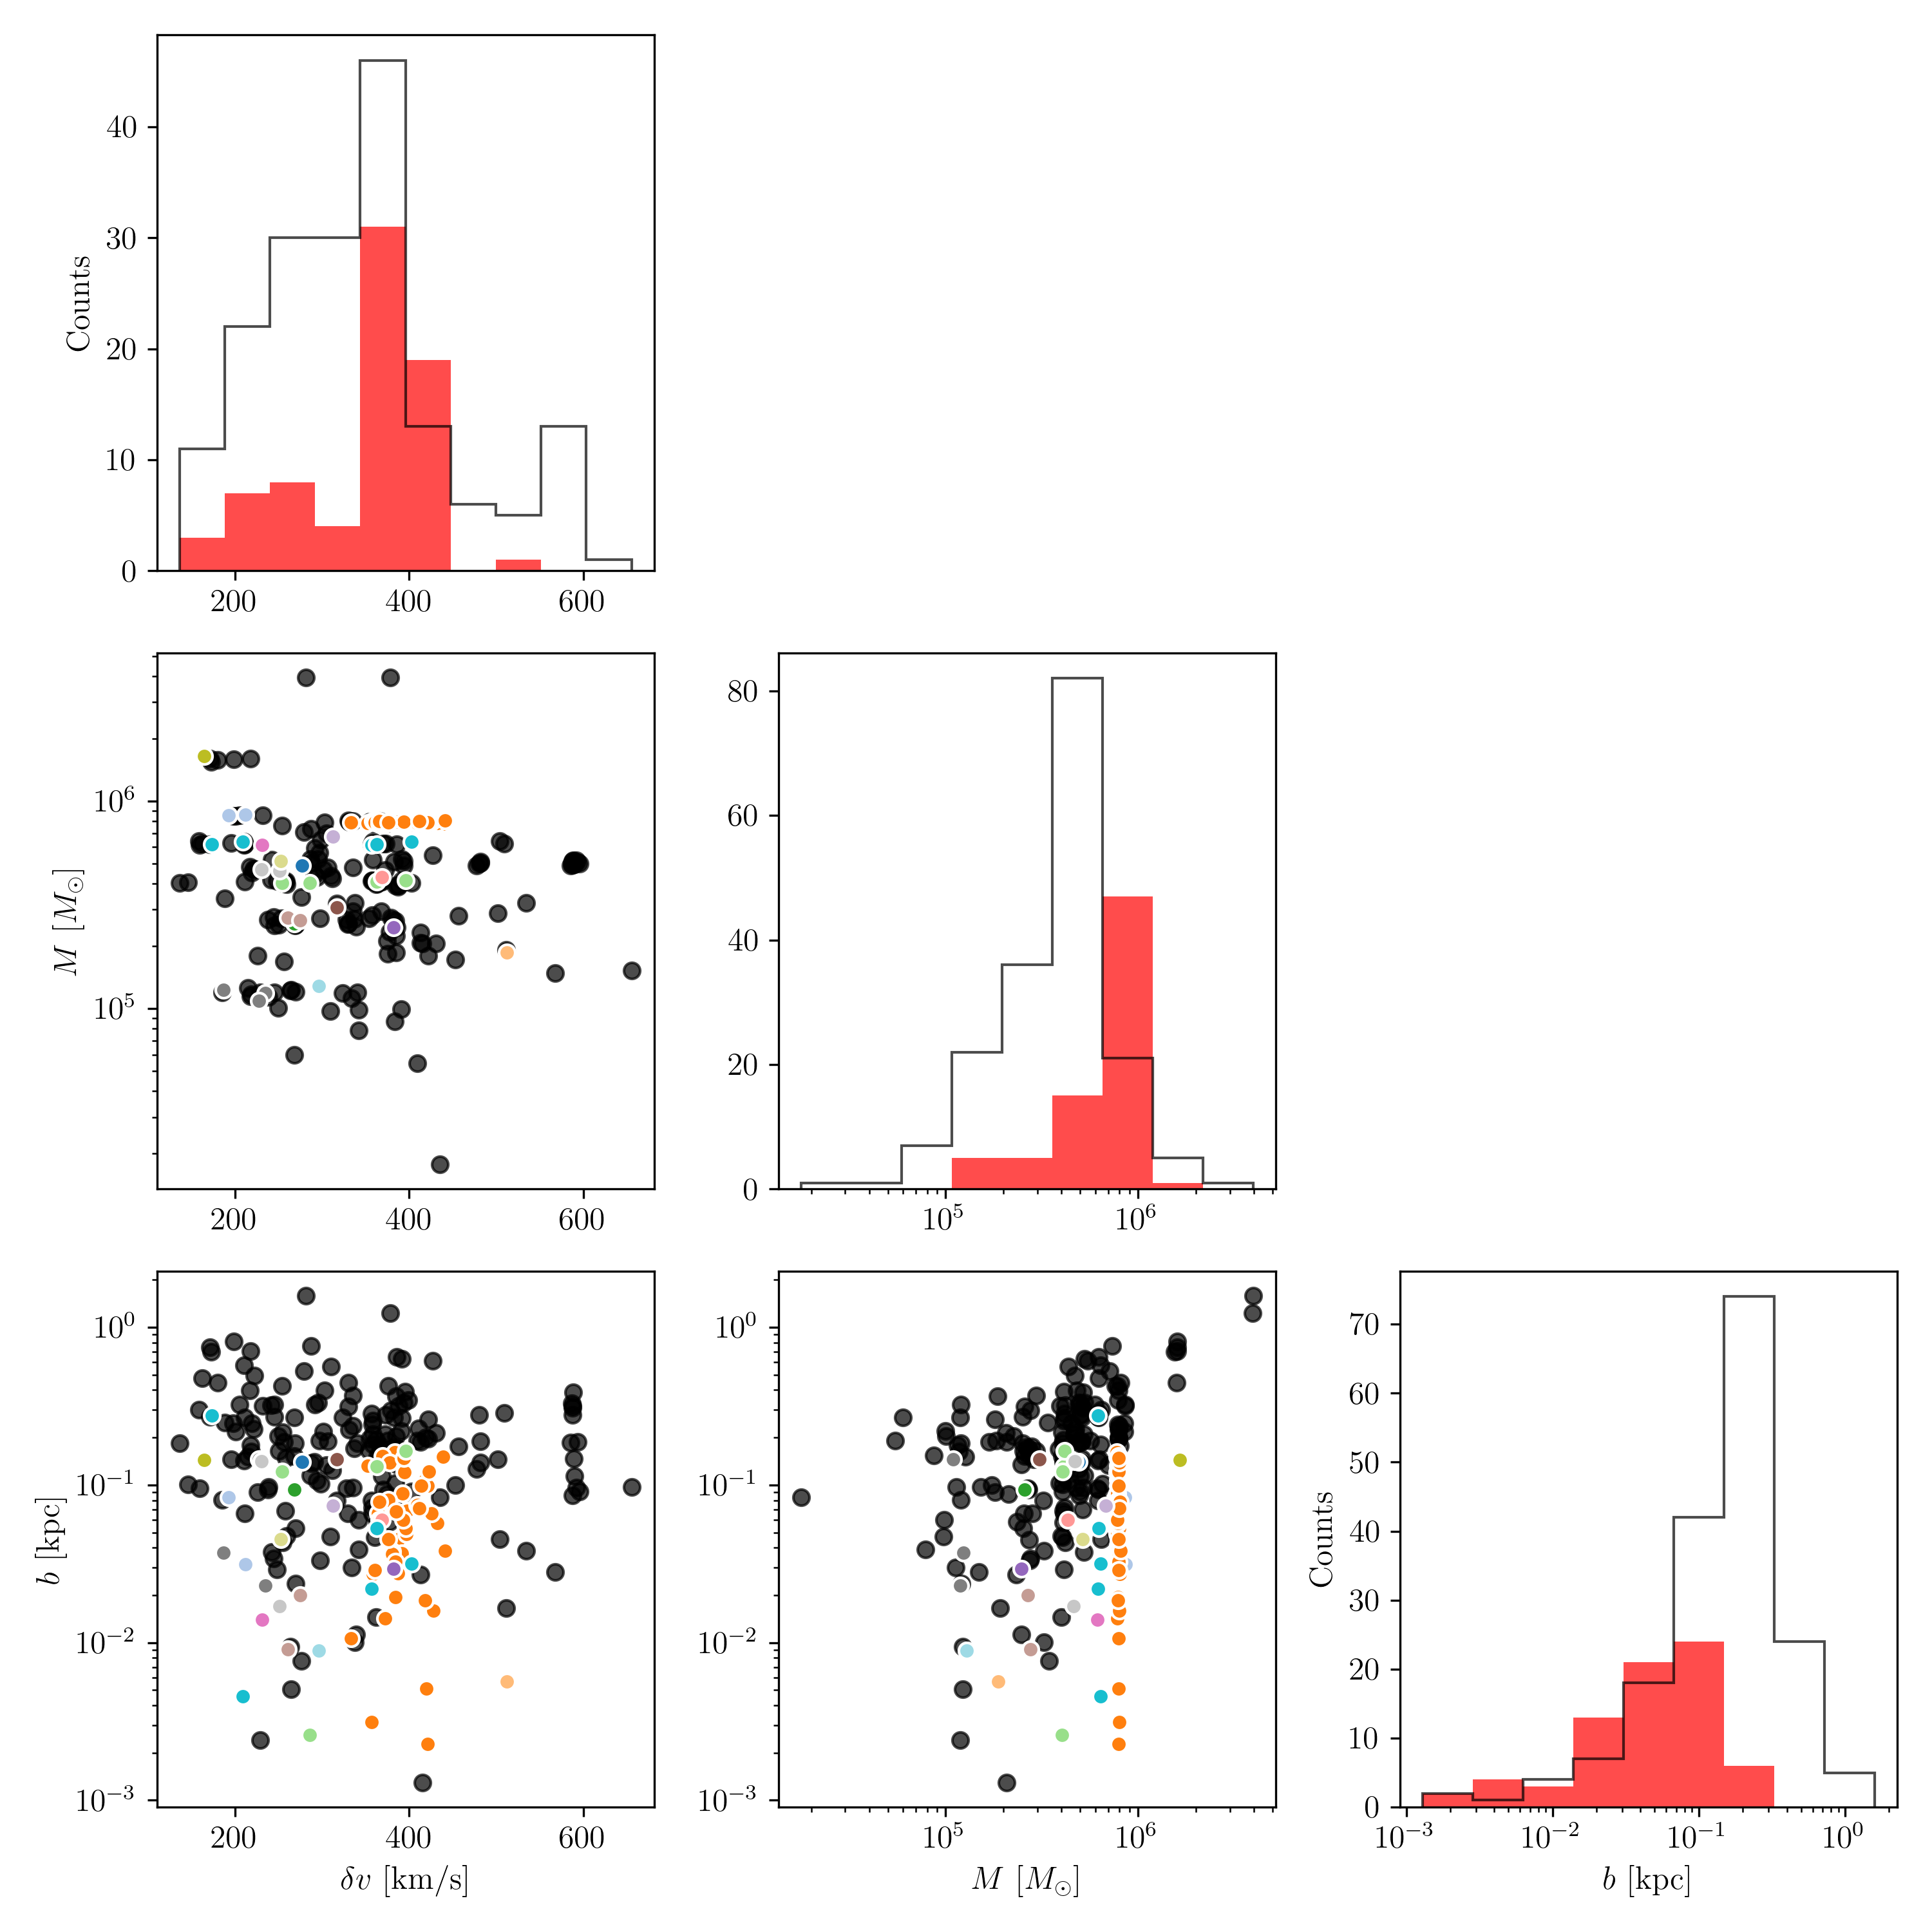
\includegraphics[width=\linewidth]{impact_geometry_statistics.png}
            \caption{Distribution and relationship between the impact variables from Eq.~\ref{eq:change_in_momentum} for all close flybys considered. The colors indicate the encounters that cause gaps and are the same as Fig.~\ref{fig:histogram_impact_time}, with white edges for visibility and binned in red for the histograms. The black histogram shows the close encounters that did not lead to gaps. Indeed, no obvious trend has emerged that delimits these planes into gap-producing or non-gap-producing ones.}
            \label{fig:impact_geometry_statistics}    
        \end{figure*}    

        With the perturbers identified, we perform statistical analysis to understand the conditions necessary for a globular cluster to induce a gap in the Palomar~5 stream. We turn to impact theory, which in its simplest form is presented in works such as \citet{2008gady.book.....B}. Consider two particles: one stationary and the other moving past it. The impact parameter is the distance between the two particles at the point of their closest approach. The impulse approximation is employed, which assumes that the velocity of the perturber remains unchanged during the interaction. This assumption simplifies the computation.

        To understand how the impacted particle is perturbed, one needs to compute its change in momentum, which is determined by integrating the force acting on the particle throughout the interaction. A useful approximation for this change in momentum, per unit mass, is the force at the closest approach multiplied by an estimate of the interaction time:
        \begin{equation} \label{eq:change_in_momentum} \Delta p \approx \text{Force} \times \text{interaction time} = \frac{GM}{b^2} \times 2\frac{b}{\delta v} = 2\frac{GM}{b \delta v}, \end{equation}where $M$ is the mass of the perturber, $b$ is the impact parameter, $\delta v$ is the relative velocity of the perturber with respect to the particle, and $G$ is the gravitational constant. 

        This equation asserts that a more massive perturber, passing closer to the particle and moving more slowly, will have a greater impact. It is important to note that the momentum change is inversely proportional to the velocity of the perturber. Note that this contrasts with the intuition from elastic collisions, such as those between billiard balls, where higher velocities result in greater impacts.

        \citet{2015MNRAS.450.1136E} extended this impact theory from one point mass impacting another to studying how an extended body impacts a stream by quantifying the change in momentum of a given particle as a function of its distance from the point of greatest impact along the stream. \citet{2015MNRAS.450.1136E} models their perturber as a Plummer sphere, like in our simulations. Since a stream is not a point but has length and an orientation in space, one needs to consider the parallel and perpendicular components of the velocity to describe the impact fully. Consequently, five parameters determine the change in velocity of a given stream particle: $M$, $r_p$, $b$, $W_\parallel$, and $W_\perp$, which are the mass of the perturber, size of the perturber, impact parameter, parallel and perpendicular components of the relative velocity. As detailed in Appendix~\ref{sec:reconstruction}, we calculated these parameters for all our \texttt{full} simulations by selecting -- for each of them --  the strongest five flybys of a perturber with the Palomar~5 stream. Thus, we compute 250 impacts and flag those that give way to gaps. 

        Visual inspection of the five key impact parameters ($M$, $r_p$, $b$, $W_\parallel$, and $W_\perp$) did not reveal a clear distinction between flybys that create gaps and those that do not. Therefore, we only present the quantities from Eq.~\ref{eq:change_in_momentum} in Fig.~\ref{fig:impact_geometry_statistics}. 
    
        Note that this figure displays the total relative velocity rather than separating the parallel and perpendicular components, as no specific trends were observed when plotting the two velocity components separately. We also excluded the characteristic cluster radius, which showed little correlation with the results, likely due to the narrow range of globular cluster radii (see Fig.~\ref{fig:mass_size_plane}). This factor might be more significant for dark matter subhalos, where size variation is greater.      
  
        While Fig.~\ref{fig:impact_geometry_statistics} demonstrates that mass, relative velocity, or impact parameter alone cannot predict gap formation, one interesting result emerges: impact parameters greater than 300~pc do not create gaps. The stream widths are roughly 200~pc, as seen in the \href{https://doi.org/10.5281/zenodo.15528089}{online appendix}. This finding is even more evident when examining the $b$-$M$ plane. A series of perturbers at roughly $\sim8 \times 10^5 M_\odot$ highlights NGC~2808's flybys, where all encounters with impact parameters under 200~pc result in gaps, while those beyond this distance do not. In other words, even the most massive globular clusters with masses greater than about $10^6 M_\odot$ cannot cause gaps if their impact parameters are greater than roughly $300$~pc. Interestingly, even fast encounters ($\delta v > 300$~km/s) can produce gaps for impact parameter values below this threshold. Perhaps this is not surprising, since the range of possible relative velocities is much less than that of mass and impact parameters, which vary by two and three orders of magnitude, respectively. In contrast, the relative velocities only vary by about a factor of three.

        \begin{figure}
            \centering
            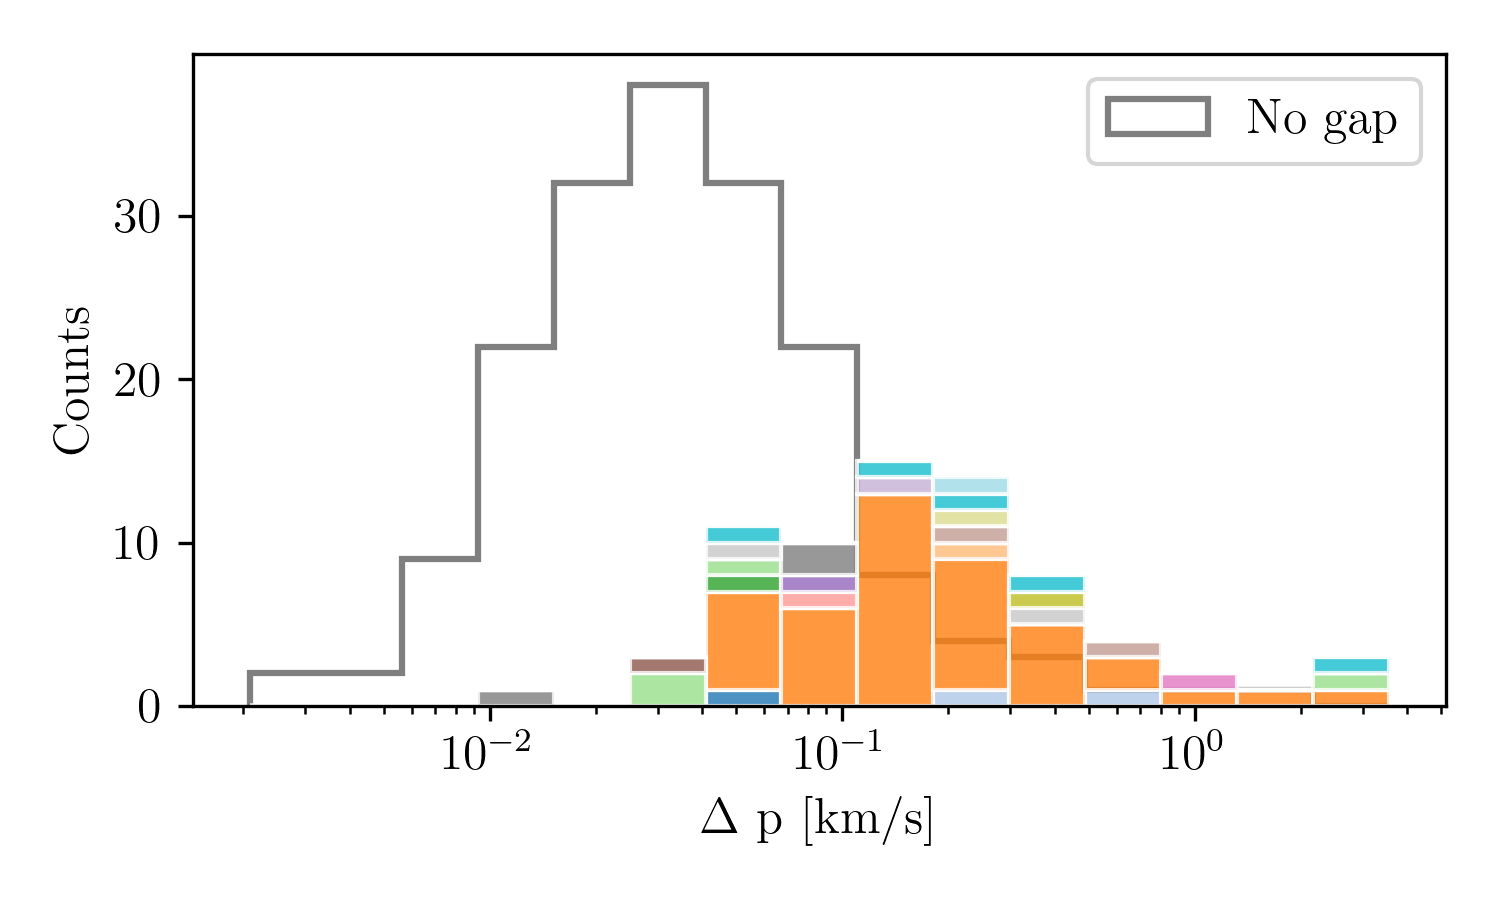
\includegraphics[width=1\linewidth]{impact_geometry_statistics_deltaP.png}
            \caption{Distribution of imparted change in momentum (per unit mass) from a cluster flyby given by Eq.~\ref{eq:change_in_momentum}. The data set includes the top 5 strongest flybys from each simulation. Those that cause gaps are colored, stacked, and overlaid atop those that do not — this is the gray distribution. We note the meaning of the colors is the same as in Fig.~\ref{fig:histogram_impact_time}.}
            \label{fig:deltap}
        \end{figure}

        \begin{figure*}
            \centering
            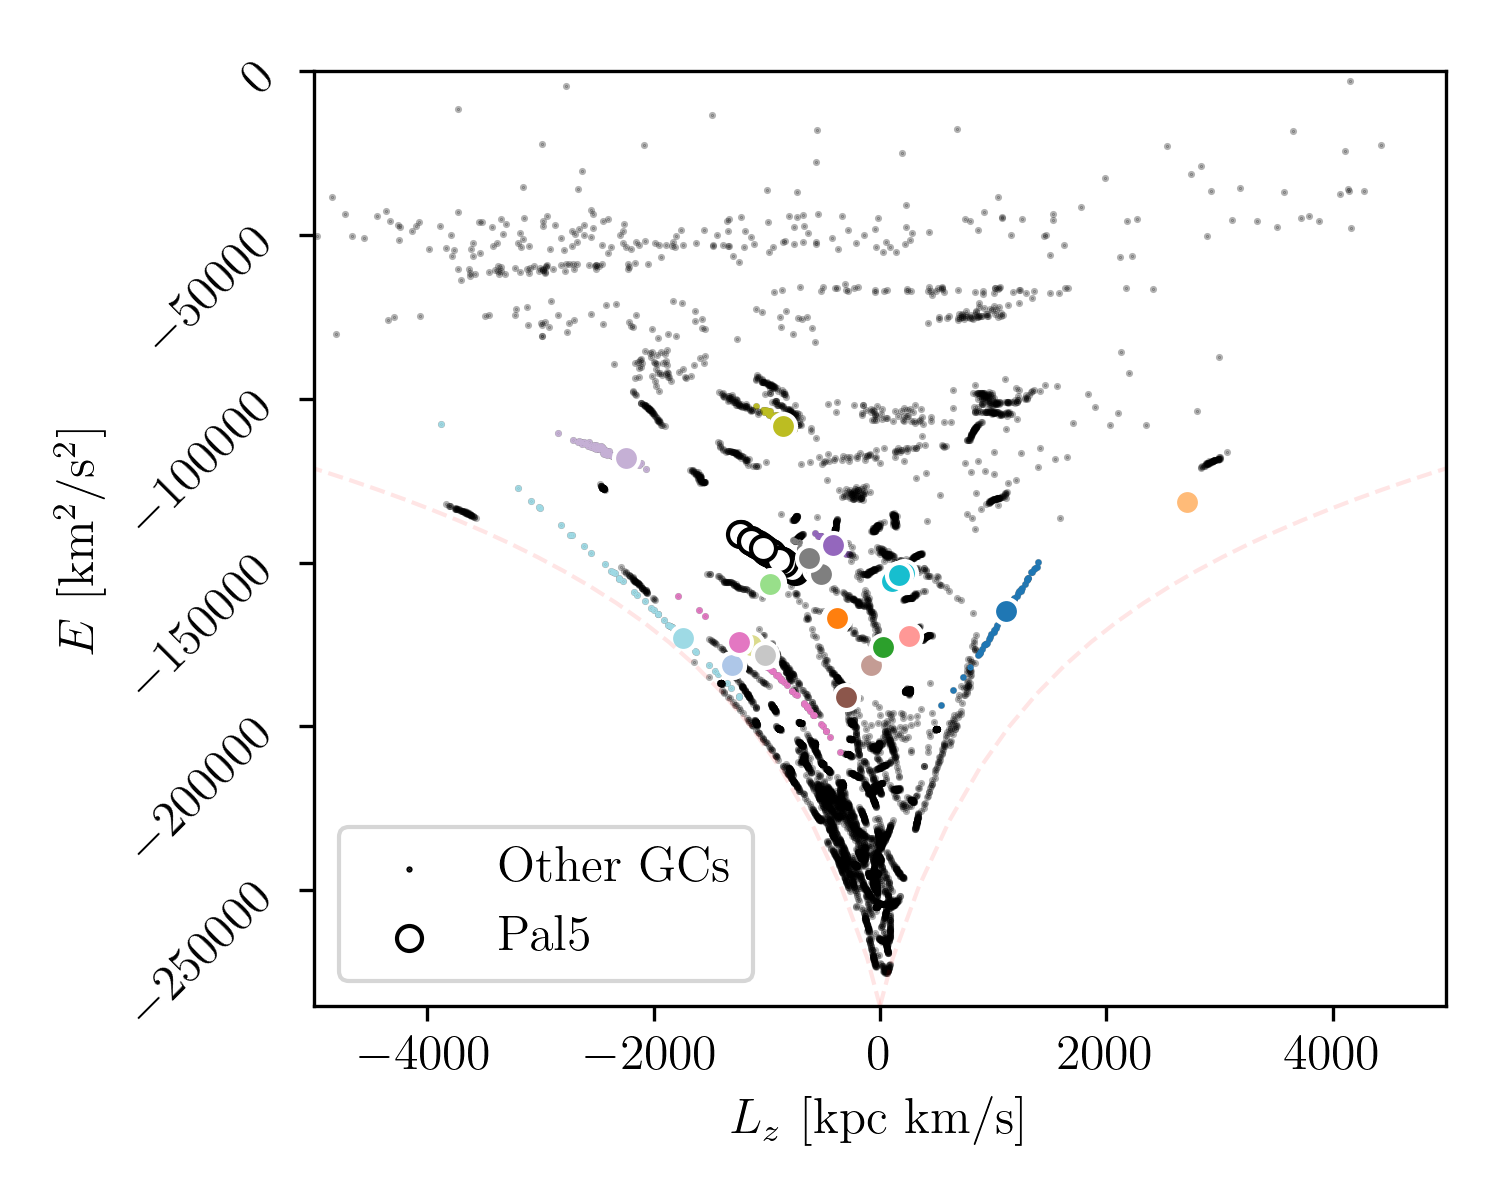
\includegraphics[width=0.45\linewidth]{E_Lz_perturbers.png}
            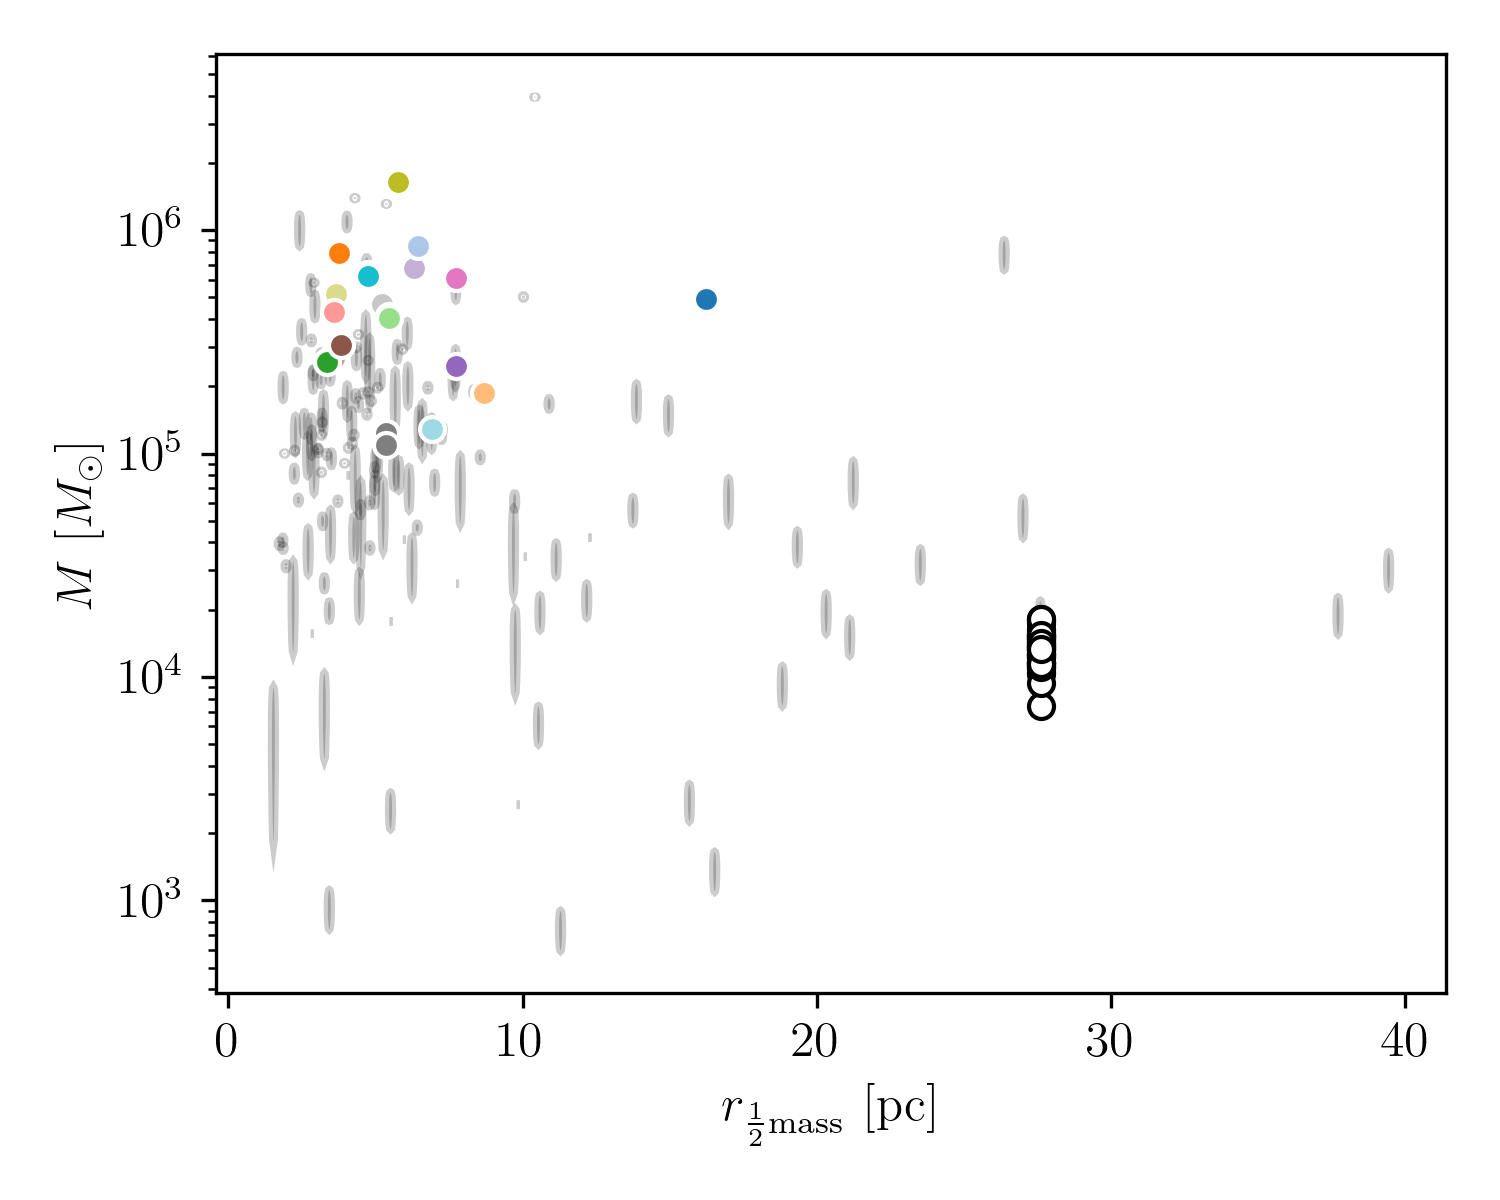
\includegraphics[width=0.45\linewidth]{mass_size_plane.png}
            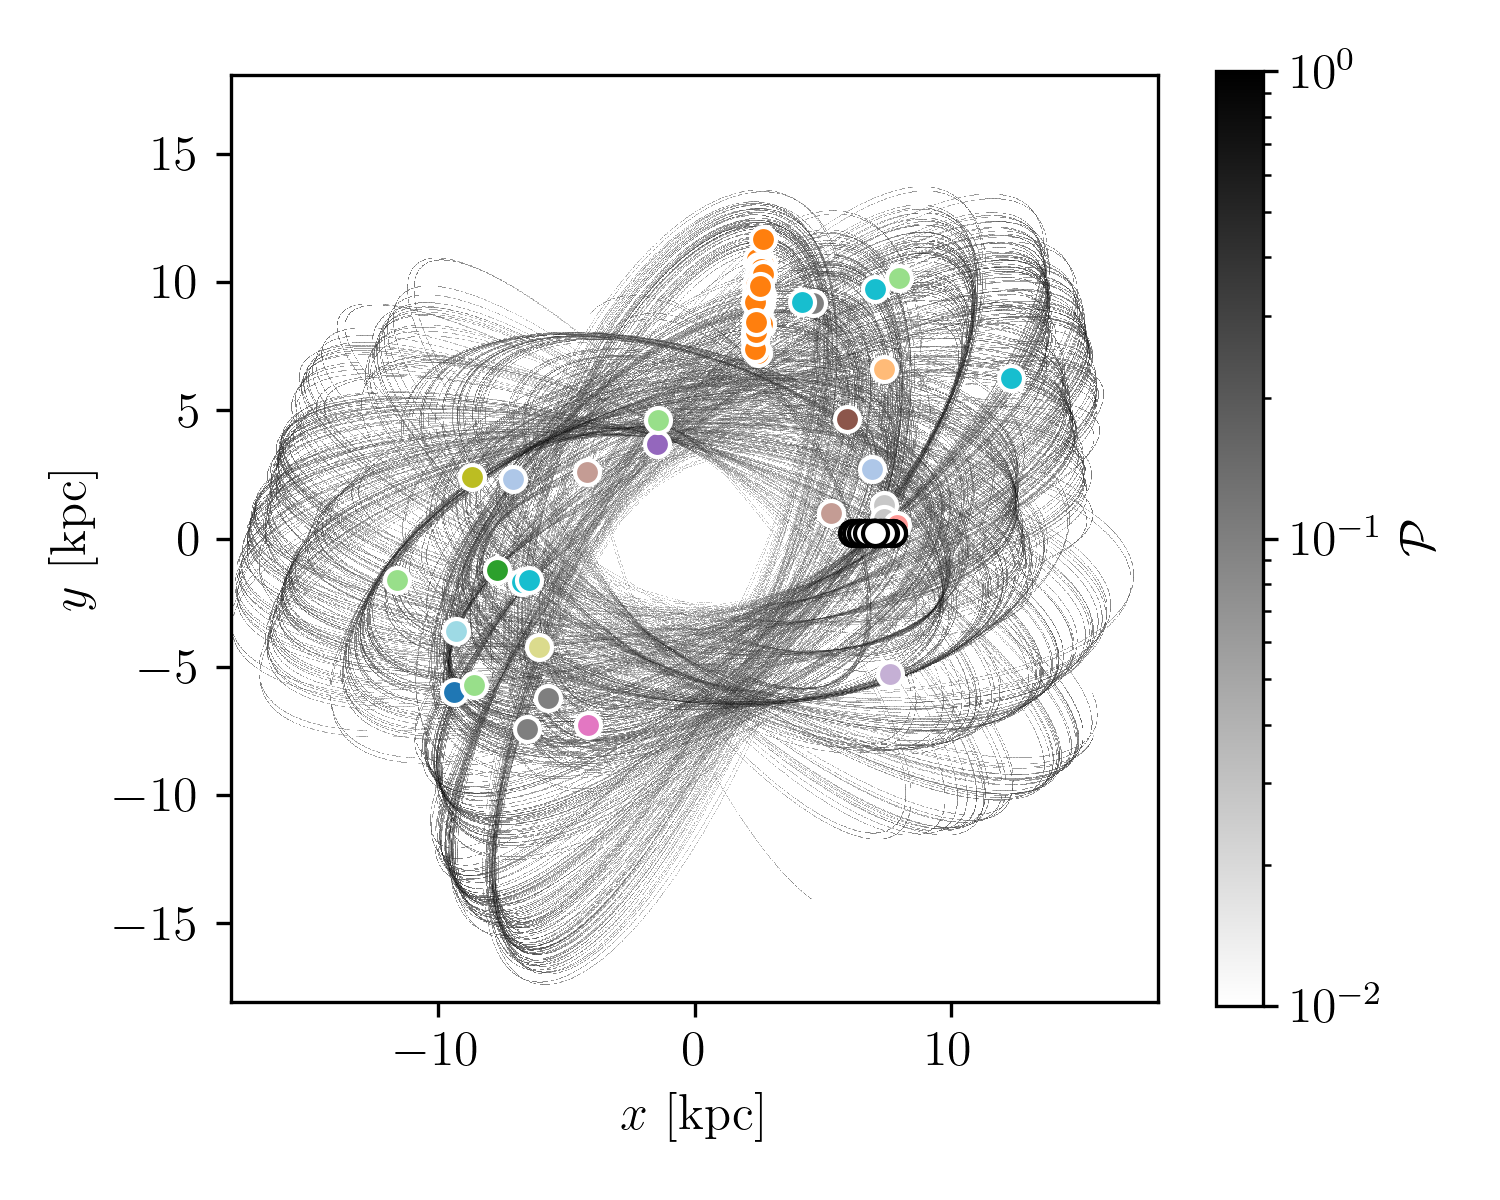
\includegraphics[width=0.45\linewidth]{impact_stats_phase_space_xy.png}
            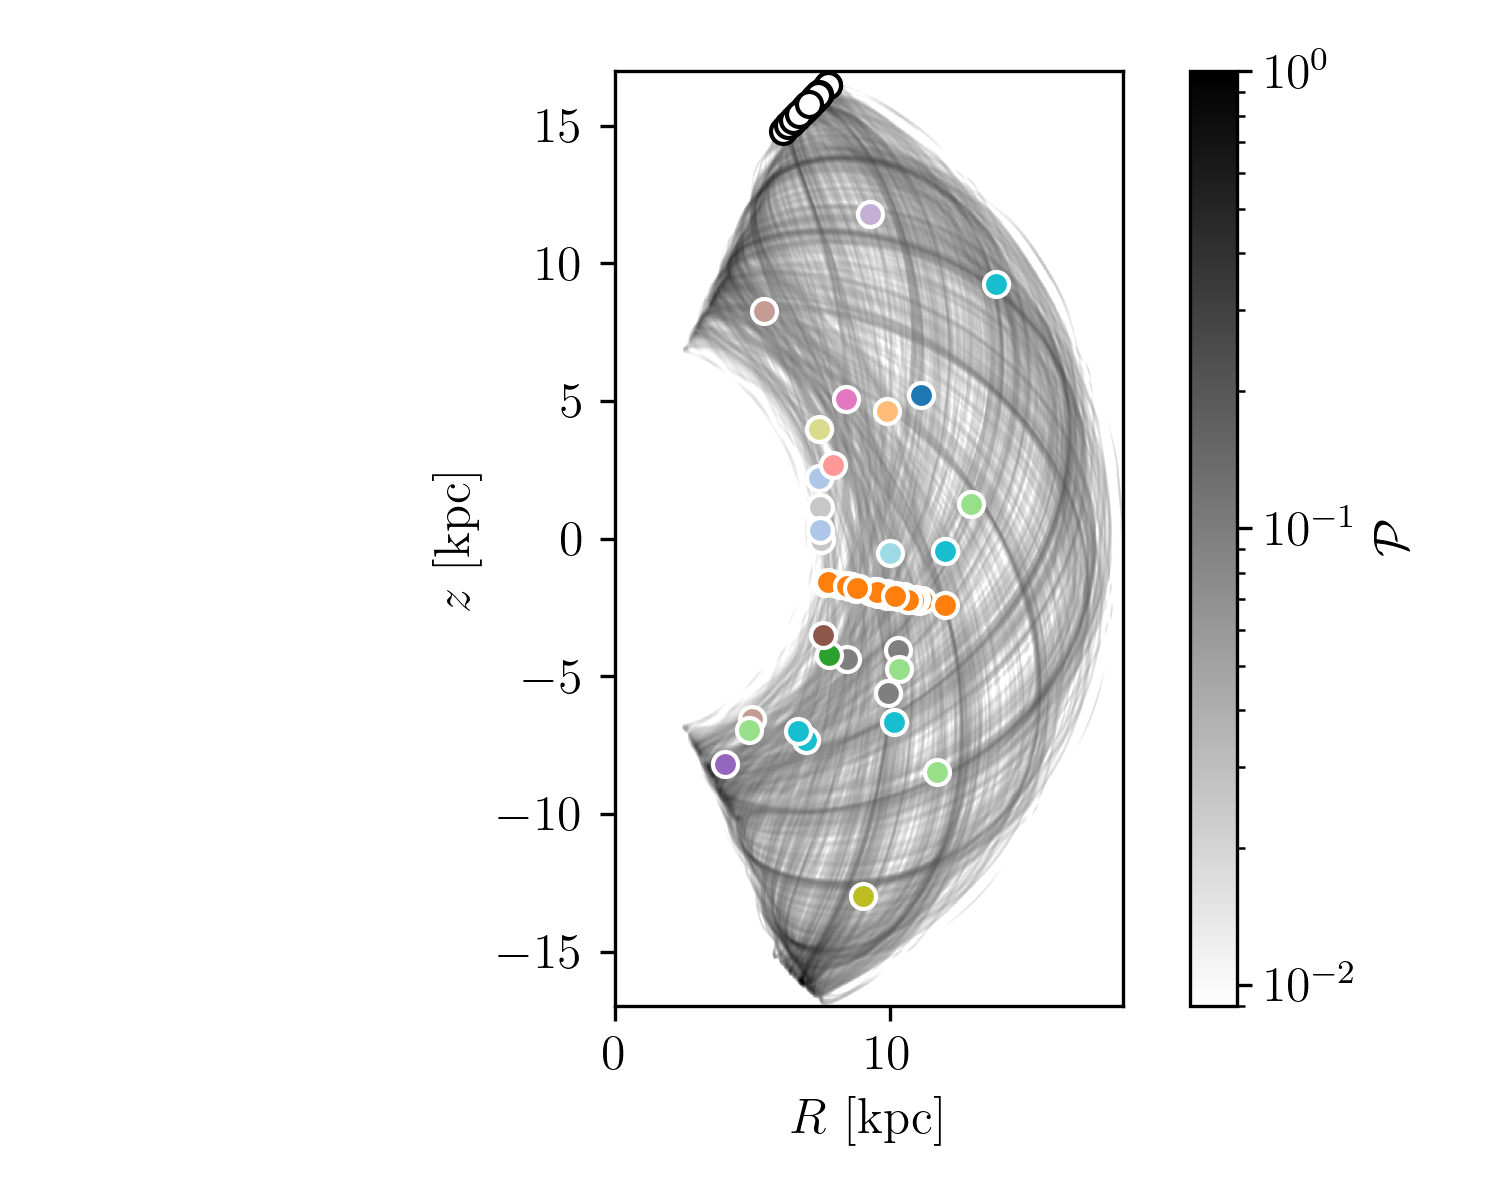
\includegraphics[width=0.45\linewidth]{impact_stats_phase_space.png}
            \caption{\textit{Top left:} Energy-angular momentum space of the globular clusters in the simulations, with 50~$\times$~165 data points representing all sampled initial conditions. Clusters impacting Palomar~5 are shown with colored markers, large for the samplings that induce a gap and small for those that do not. The small gray dots represent the non-gap-causing clusters. The 50 white dots indicate Palomar~5's sampled initial conditions for the current day position. The light-pink dashed curve shows the circular velocity curve. \textit{Top right:} Mass-size plane of the globular clusters in the simulations, with uncertainties on the masses indicated as vertical lines. We remind the reader that the globular cluster catalog currently does not provide uncertainties for the characteristic radii of clusters. \textit{Bottom left:} Palomar~5's orbit in the Galactocentric xy plane. The gray scale represents all 50 stacked orbits, with $\mathcal{P}$ indicating the probability of Palomar~5's position, normalized to $\mathcal{P}_\textrm{max}=1$. The colored markers indicate the position of the perturber when it impacted the stream and \textit{not} its present-day position. \textit{Bottom right:} Same as the bottom left but in the meridional plane. In all panels, the colors of the markers and histogram bars correspond to specific perturbers as specified in Fig.~\ref{fig:histogram_impact_time}.}
            \label{fig:mass_size_plane}
        \end{figure*}        
      



\section{Velocity distribution within the stream}

    \subsection{Self-Segregation and Stream Chilling}

    The classic collisionless boltzmann equation:
    \begin{equation}
        \frac{df}{dt} = 0 = \frac{\partial f}{\partial x} \frac{dx}{dt} + \frac{\partial f}{\partial v} \frac{dv}{dt}+ \frac{\partial f}{\partial t} 
    \end{equation}

    we are saying that the pusles drift with the same velocities thus $\frac{dv}{dt}=0$. I impart more assumptions, namely that: $\rho(x,t=0)=\delta(x)$ and that velocity is defined as a normal distribution that does not change over time. This means that I can write the initial distribution function as:
    
    \begin{equation}
        f(x,v,t=0) = \delta(x)\frac{1}{\sigma\sqrt{2\pi}}\textrm{exp}\left(-\frac{1}{2}\left(\frac{v-\langle v \rangle}{\sigma}\right)^2\right)
    \end{equation}    

    the solution to the evolution of the density is $\rho = \int f dv$, and you also need to perform this variable substitution $f(x,v,t) = f(x-vt,v,0)$

    \begin{equation}
        \rho(x,t) = \frac{1}{\sigma t \sqrt{2\pi} }\textrm{exp}\left(-\frac{1}{2}\left(\frac{x-\langle v \rangle t}{\sigma_v t}\right)^2\right)
    \end{equation}

    it's also useful to know the relative velocity of the impact site between one group and another. These things drift apart. How much faster does one group go ahead of another? 
    \begin{equation}
        \delta v_{ij} = \frac{x\prime}{t-iT} - \frac{x\prime}{t-jT}
    \end{equation}
    where $i,j$ are the indexes for the packet. Note that this only works for $t > nT$ where $T$ is the orbital period, or spacing between the impacts, $n$ is the number of pericenter passages. $t$ is the total simulation time. $x\prime$ is the position of the impact. It makes sense that the velocity of the particle is the position where the impact occured, divided by the time since it left the origin. 